% Created by tikzDevice version 0.12.6 on 2026-07-06 23:55:43
% !TEX encoding = UTF-8 Unicode
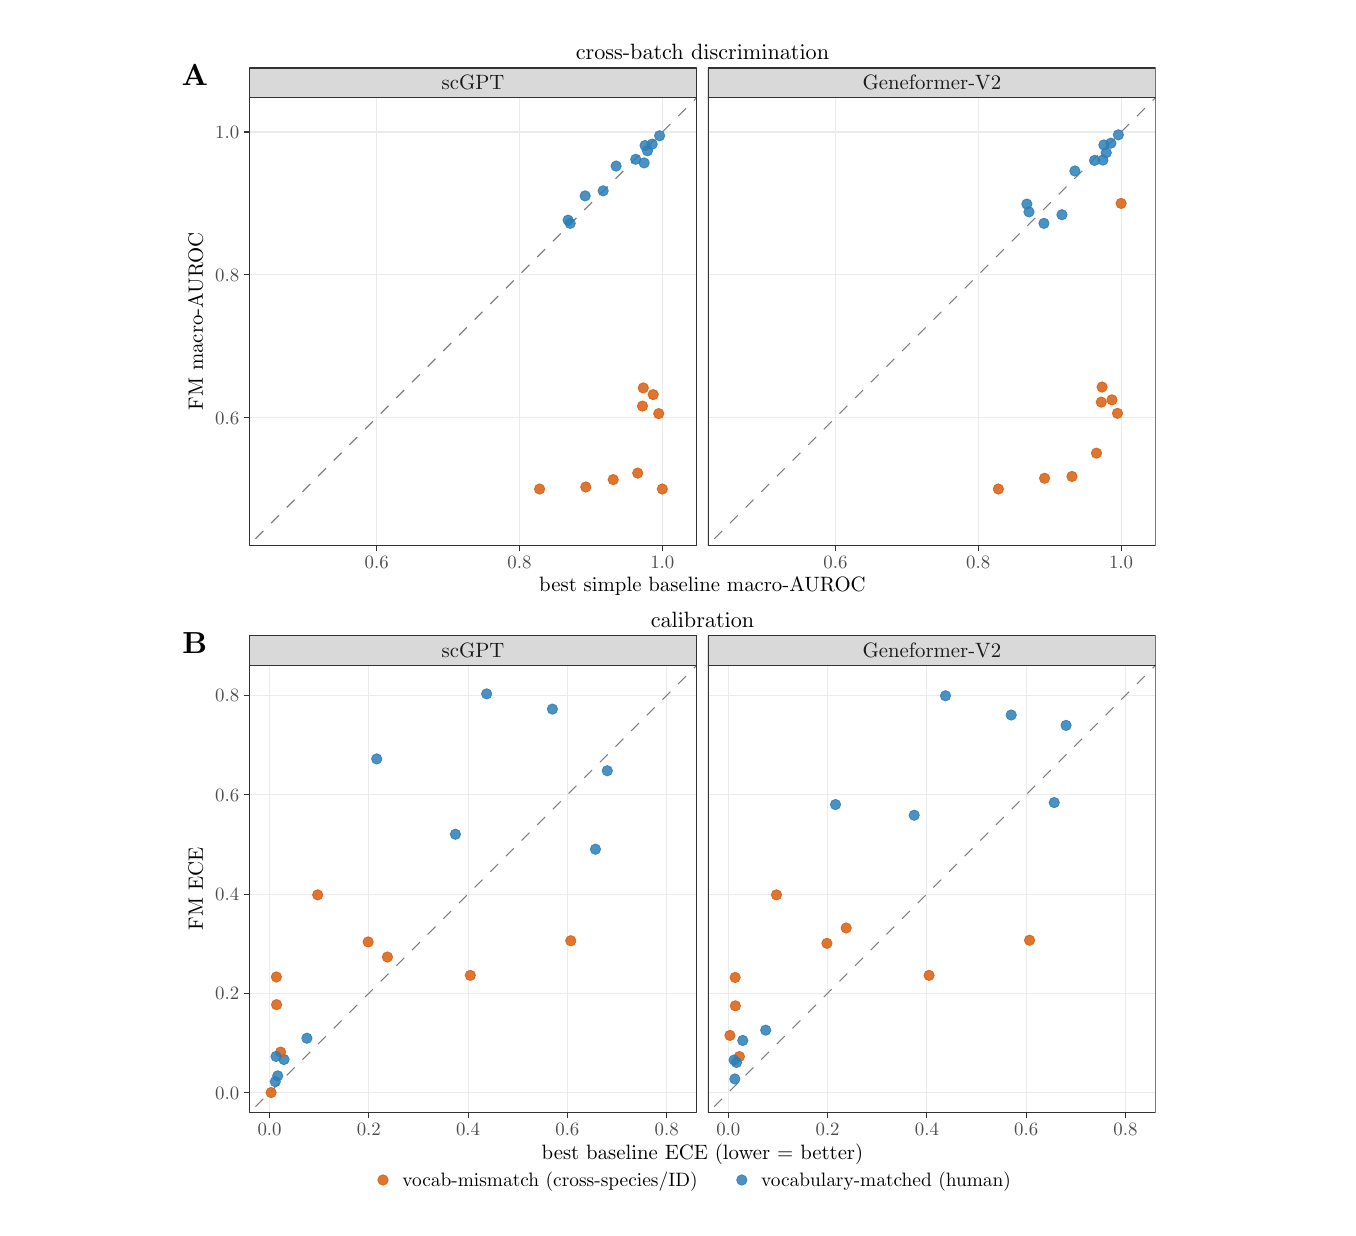
\begin{tikzpicture}[x=1pt,y=1pt]
\definecolor{fillColor}{RGB}{255,255,255}
\path[use as bounding box,fill=fillColor,fill opacity=0.00] (0,0) rectangle (469.75,426.39);
\begin{scope}
\path[clip] (  0.00,  0.00) rectangle (469.75,426.39);
\definecolor{drawColor}{RGB}{255,255,255}
\definecolor{fillColor}{RGB}{255,255,255}

\path[draw=drawColor,line width= 0.4pt,line join=round,line cap=round,fill=fillColor] ( -0.00,  0.00) rectangle (469.76,426.39);
\end{scope}
\begin{scope}
\path[clip] (  4.00,218.20) rectangle (463.75,423.39);
\definecolor{drawColor}{RGB}{255,255,255}
\definecolor{fillColor}{RGB}{255,255,255}

\path[draw=drawColor,line width= 0.4pt,line join=round,line cap=round,fill=fillColor] (  4.00,218.20) rectangle (463.75,423.39);
\end{scope}
\begin{scope}
\path[clip] (  4.00,  3.00) rectangle (463.75,218.20);
\definecolor{drawColor}{RGB}{255,255,255}
\definecolor{fillColor}{RGB}{255,255,255}

\path[draw=drawColor,line width= 0.4pt,line join=round,line cap=round,fill=fillColor] (  4.00,  3.00) rectangle (463.75,218.20);
\end{scope}
\begin{scope}
\path[clip] ( 80.05,239.43) rectangle (241.83,401.20);
\definecolor{fillColor}{RGB}{255,255,255}

\path[fill=fillColor] ( 80.05,239.42) rectangle (241.83,401.20);
\definecolor{drawColor}{gray}{0.92}

\path[draw=drawColor,line width= 0.4pt,line join=round] ( 80.05,285.48) --
	(241.83,285.48);

\path[draw=drawColor,line width= 0.4pt,line join=round] ( 80.05,337.09) --
	(241.83,337.09);

\path[draw=drawColor,line width= 0.4pt,line join=round] ( 80.05,388.69) --
	(241.83,388.69);

\path[draw=drawColor,line width= 0.4pt,line join=round] (126.11,239.43) --
	(126.11,401.20);

\path[draw=drawColor,line width= 0.4pt,line join=round] (177.71,239.43) --
	(177.71,401.20);

\path[draw=drawColor,line width= 0.4pt,line join=round] (229.32,239.43) --
	(229.32,401.20);
\definecolor{drawColor}{gray}{0.50}

\path[draw=drawColor,line width= 0.4pt,dash pattern=on 4pt off 4pt ,line join=round] (-81.73, 77.65) -- (403.61,562.98);
\definecolor{drawColor}{RGB}{44,127,184}
\definecolor{fillColor}{RGB}{44,127,184}

\path[draw=drawColor,draw opacity=0.85,line width= 0.3pt,line join=round,line cap=round,fill=fillColor,fill opacity=0.85] (223.97,381.91) circle (  1.87);

\path[draw=drawColor,draw opacity=0.85,line width= 0.3pt,line join=round,line cap=round,fill=fillColor,fill opacity=0.85] (196.04,355.67) circle (  1.87);
\definecolor{drawColor}{RGB}{217,95,14}
\definecolor{fillColor}{RGB}{217,95,14}

\path[draw=drawColor,draw opacity=0.85,line width= 0.3pt,line join=round,line cap=round,fill=fillColor,fill opacity=0.85] (222.16,289.65) circle (  1.87);
\definecolor{drawColor}{RGB}{44,127,184}
\definecolor{fillColor}{RGB}{44,127,184}

\path[draw=drawColor,draw opacity=0.85,line width= 0.3pt,line join=round,line cap=round,fill=fillColor,fill opacity=0.85] (195.28,356.84) circle (  1.87);

\path[draw=drawColor,draw opacity=0.85,line width= 0.3pt,line join=round,line cap=round,fill=fillColor,fill opacity=0.85] (207.95,367.43) circle (  1.87);
\definecolor{drawColor}{RGB}{217,95,14}
\definecolor{fillColor}{RGB}{217,95,14}

\path[draw=drawColor,draw opacity=0.85,line width= 0.3pt,line join=round,line cap=round,fill=fillColor,fill opacity=0.85] (222.45,296.21) circle (  1.87);
\definecolor{drawColor}{RGB}{44,127,184}
\definecolor{fillColor}{RGB}{44,127,184}

\path[draw=drawColor,draw opacity=0.85,line width= 0.3pt,line join=round,line cap=round,fill=fillColor,fill opacity=0.85] (222.76,377.51) circle (  1.87);
\definecolor{drawColor}{RGB}{217,95,14}
\definecolor{fillColor}{RGB}{217,95,14}

\path[draw=drawColor,draw opacity=0.85,line width= 0.3pt,line join=round,line cap=round,fill=fillColor,fill opacity=0.85] (226.03,293.80) circle (  1.87);
\definecolor{drawColor}{RGB}{44,127,184}
\definecolor{fillColor}{RGB}{44,127,184}

\path[draw=drawColor,draw opacity=0.85,line width= 0.3pt,line join=round,line cap=round,fill=fillColor,fill opacity=0.85] (212.62,376.38) circle (  1.87);

\path[draw=drawColor,draw opacity=0.85,line width= 0.3pt,line join=round,line cap=round,fill=fillColor,fill opacity=0.85] (201.44,365.61) circle (  1.87);

\path[draw=drawColor,draw opacity=0.85,line width= 0.3pt,line join=round,line cap=round,fill=fillColor,fill opacity=0.85] (223.09,383.81) circle (  1.87);

\path[draw=drawColor,draw opacity=0.85,line width= 0.3pt,line join=round,line cap=round,fill=fillColor,fill opacity=0.85] (219.73,378.83) circle (  1.87);
\definecolor{drawColor}{RGB}{217,95,14}
\definecolor{fillColor}{RGB}{217,95,14}

\path[draw=drawColor,draw opacity=0.85,line width= 0.3pt,line join=round,line cap=round,fill=fillColor,fill opacity=0.85] (229.32,259.68) circle (  1.87);

\path[draw=drawColor,draw opacity=0.85,line width= 0.3pt,line join=round,line cap=round,fill=fillColor,fill opacity=0.85] (184.97,259.68) circle (  1.87);

\path[draw=drawColor,draw opacity=0.85,line width= 0.3pt,line join=round,line cap=round,fill=fillColor,fill opacity=0.85] (220.43,265.43) circle (  1.87);
\definecolor{drawColor}{RGB}{44,127,184}
\definecolor{fillColor}{RGB}{44,127,184}

\path[draw=drawColor,draw opacity=0.85,line width= 0.3pt,line join=round,line cap=round,fill=fillColor,fill opacity=0.85] (228.34,387.33) circle (  1.87);
\definecolor{drawColor}{RGB}{217,95,14}
\definecolor{fillColor}{RGB}{217,95,14}

\path[draw=drawColor,draw opacity=0.85,line width= 0.3pt,line join=round,line cap=round,fill=fillColor,fill opacity=0.85] (211.58,263.08) circle (  1.87);
\definecolor{drawColor}{RGB}{44,127,184}
\definecolor{fillColor}{RGB}{44,127,184}

\path[draw=drawColor,draw opacity=0.85,line width= 0.3pt,line join=round,line cap=round,fill=fillColor,fill opacity=0.85] (225.65,384.31) circle (  1.87);
\definecolor{drawColor}{RGB}{217,95,14}
\definecolor{fillColor}{RGB}{217,95,14}

\path[draw=drawColor,draw opacity=0.85,line width= 0.3pt,line join=round,line cap=round,fill=fillColor,fill opacity=0.85] (228.02,286.93) circle (  1.87);

\path[draw=drawColor,draw opacity=0.85,line width= 0.3pt,line join=round,line cap=round,fill=fillColor,fill opacity=0.85] (201.67,260.41) circle (  1.87);
\definecolor{drawColor}{gray}{0.20}

\path[draw=drawColor,line width= 0.4pt,line join=round,line cap=round] ( 80.05,239.42) rectangle (241.83,401.20);
\end{scope}
\begin{scope}
\path[clip] (245.83,239.43) rectangle (407.61,401.20);
\definecolor{fillColor}{RGB}{255,255,255}

\path[fill=fillColor] (245.83,239.42) rectangle (407.61,401.20);
\definecolor{drawColor}{gray}{0.92}

\path[draw=drawColor,line width= 0.4pt,line join=round] (245.83,285.48) --
	(407.61,285.48);

\path[draw=drawColor,line width= 0.4pt,line join=round] (245.83,337.09) --
	(407.61,337.09);

\path[draw=drawColor,line width= 0.4pt,line join=round] (245.83,388.69) --
	(407.61,388.69);

\path[draw=drawColor,line width= 0.4pt,line join=round] (291.89,239.43) --
	(291.89,401.20);

\path[draw=drawColor,line width= 0.4pt,line join=round] (343.49,239.43) --
	(343.49,401.20);

\path[draw=drawColor,line width= 0.4pt,line join=round] (395.10,239.43) --
	(395.10,401.20);
\definecolor{drawColor}{gray}{0.50}

\path[draw=drawColor,line width= 0.4pt,dash pattern=on 4pt off 4pt ,line join=round] ( 84.05, 77.65) -- (569.39,562.98);
\definecolor{drawColor}{RGB}{44,127,184}
\definecolor{fillColor}{RGB}{44,127,184}

\path[draw=drawColor,draw opacity=0.85,line width= 0.3pt,line join=round,line cap=round,fill=fillColor,fill opacity=0.85] (389.74,381.21) circle (  1.87);

\path[draw=drawColor,draw opacity=0.85,line width= 0.3pt,line join=round,line cap=round,fill=fillColor,fill opacity=0.85] (361.82,359.82) circle (  1.87);
\definecolor{drawColor}{RGB}{217,95,14}
\definecolor{fillColor}{RGB}{217,95,14}

\path[draw=drawColor,draw opacity=0.85,line width= 0.3pt,line join=round,line cap=round,fill=fillColor,fill opacity=0.85] (387.94,291.08) circle (  1.87);
\definecolor{drawColor}{RGB}{44,127,184}
\definecolor{fillColor}{RGB}{44,127,184}

\path[draw=drawColor,draw opacity=0.85,line width= 0.3pt,line join=round,line cap=round,fill=fillColor,fill opacity=0.85] (361.06,362.64) circle (  1.87);

\path[draw=drawColor,draw opacity=0.85,line width= 0.3pt,line join=round,line cap=round,fill=fillColor,fill opacity=0.85] (373.73,358.79) circle (  1.87);
\definecolor{drawColor}{RGB}{217,95,14}
\definecolor{fillColor}{RGB}{217,95,14}

\path[draw=drawColor,draw opacity=0.85,line width= 0.3pt,line join=round,line cap=round,fill=fillColor,fill opacity=0.85] (388.23,296.53) circle (  1.87);
\definecolor{drawColor}{RGB}{44,127,184}
\definecolor{fillColor}{RGB}{44,127,184}

\path[draw=drawColor,draw opacity=0.85,line width= 0.3pt,line join=round,line cap=round,fill=fillColor,fill opacity=0.85] (388.54,378.55) circle (  1.87);
\definecolor{drawColor}{RGB}{217,95,14}
\definecolor{fillColor}{RGB}{217,95,14}

\path[draw=drawColor,draw opacity=0.85,line width= 0.3pt,line join=round,line cap=round,fill=fillColor,fill opacity=0.85] (391.81,291.90) circle (  1.87);
\definecolor{drawColor}{RGB}{44,127,184}
\definecolor{fillColor}{RGB}{44,127,184}

\path[draw=drawColor,draw opacity=0.85,line width= 0.3pt,line join=round,line cap=round,fill=fillColor,fill opacity=0.85] (378.40,374.60) circle (  1.87);

\path[draw=drawColor,draw opacity=0.85,line width= 0.3pt,line join=round,line cap=round,fill=fillColor,fill opacity=0.85] (367.22,355.67) circle (  1.87);

\path[draw=drawColor,draw opacity=0.85,line width= 0.3pt,line join=round,line cap=round,fill=fillColor,fill opacity=0.85] (388.87,384.01) circle (  1.87);

\path[draw=drawColor,draw opacity=0.85,line width= 0.3pt,line join=round,line cap=round,fill=fillColor,fill opacity=0.85] (385.51,378.42) circle (  1.87);
\definecolor{drawColor}{RGB}{217,95,14}
\definecolor{fillColor}{RGB}{217,95,14}

\path[draw=drawColor,draw opacity=0.85,line width= 0.3pt,line join=round,line cap=round,fill=fillColor,fill opacity=0.85] (395.10,362.88) circle (  1.87);

\path[draw=drawColor,draw opacity=0.85,line width= 0.3pt,line join=round,line cap=round,fill=fillColor,fill opacity=0.85] (350.75,259.68) circle (  1.87);

\path[draw=drawColor,draw opacity=0.85,line width= 0.3pt,line join=round,line cap=round,fill=fillColor,fill opacity=0.85] (386.21,272.64) circle (  1.87);
\definecolor{drawColor}{RGB}{44,127,184}
\definecolor{fillColor}{RGB}{44,127,184}

\path[draw=drawColor,draw opacity=0.85,line width= 0.3pt,line join=round,line cap=round,fill=fillColor,fill opacity=0.85] (394.12,387.67) circle (  1.87);
\definecolor{drawColor}{RGB}{217,95,14}
\definecolor{fillColor}{RGB}{217,95,14}

\path[draw=drawColor,draw opacity=0.85,line width= 0.3pt,line join=round,line cap=round,fill=fillColor,fill opacity=0.85] (377.36,264.22) circle (  1.87);
\definecolor{drawColor}{RGB}{44,127,184}
\definecolor{fillColor}{RGB}{44,127,184}

\path[draw=drawColor,draw opacity=0.85,line width= 0.3pt,line join=round,line cap=round,fill=fillColor,fill opacity=0.85] (391.43,384.65) circle (  1.87);
\definecolor{drawColor}{RGB}{217,95,14}
\definecolor{fillColor}{RGB}{217,95,14}

\path[draw=drawColor,draw opacity=0.85,line width= 0.3pt,line join=round,line cap=round,fill=fillColor,fill opacity=0.85] (393.80,287.03) circle (  1.87);

\path[draw=drawColor,draw opacity=0.85,line width= 0.3pt,line join=round,line cap=round,fill=fillColor,fill opacity=0.85] (367.45,263.57) circle (  1.87);
\definecolor{drawColor}{gray}{0.20}

\path[draw=drawColor,line width= 0.4pt,line join=round,line cap=round] (245.83,239.42) rectangle (407.61,401.20);
\end{scope}
\begin{scope}
\path[clip] (  0.00,  0.00) rectangle (469.75,426.39);
\definecolor{drawColor}{RGB}{0,0,0}

\node[text=drawColor,anchor=base,inner sep=0pt, outer sep=0pt, scale=  1.10] at ( 60.40,405.50) {\bfseries A};
\end{scope}
\begin{scope}
\path[clip] (  0.00,  0.00) rectangle (469.75,426.39);
\definecolor{drawColor}{gray}{0.30}

\node[text=drawColor,anchor=base east,inner sep=0pt, outer sep=0pt, scale=  0.68] at ( 76.45,283.14) {0.6};

\node[text=drawColor,anchor=base east,inner sep=0pt, outer sep=0pt, scale=  0.68] at ( 76.45,334.74) {0.8};

\node[text=drawColor,anchor=base east,inner sep=0pt, outer sep=0pt, scale=  0.68] at ( 76.45,386.35) {1.0};
\end{scope}
\begin{scope}
\path[clip] (  0.00,  0.00) rectangle (469.75,426.39);
\definecolor{drawColor}{gray}{0.20}

\path[draw=drawColor,line width= 0.4pt,line join=round] ( 78.05,285.48) --
	( 80.05,285.48);

\path[draw=drawColor,line width= 0.4pt,line join=round] ( 78.05,337.09) --
	( 80.05,337.09);

\path[draw=drawColor,line width= 0.4pt,line join=round] ( 78.05,388.69) --
	( 80.05,388.69);
\end{scope}
\begin{scope}
\path[clip] (  0.00,  0.00) rectangle (469.75,426.39);
\definecolor{drawColor}{RGB}{0,0,0}

\node[text=drawColor,rotate= 90.00,anchor=base,inner sep=0pt, outer sep=0pt, scale=  0.75] at ( 63.31,320.31) {FM macro-AUROC};
\end{scope}
\begin{scope}
\path[clip] ( 80.05,401.20) rectangle (241.83,411.83);
\definecolor{drawColor}{gray}{0.20}
\definecolor{fillColor}{gray}{0.85}

\path[draw=drawColor,line width= 0.4pt,line join=round,line cap=round,fill=fillColor] ( 80.05,401.20) rectangle (241.83,411.83);
\definecolor{drawColor}{gray}{0.10}

\node[text=drawColor,anchor=base,inner sep=0pt, outer sep=0pt, scale=  0.75] at (160.94,403.93) {scGPT};
\end{scope}
\begin{scope}
\path[clip] (245.83,401.20) rectangle (407.61,411.83);
\definecolor{drawColor}{gray}{0.20}
\definecolor{fillColor}{gray}{0.85}

\path[draw=drawColor,line width= 0.4pt,line join=round,line cap=round,fill=fillColor] (245.83,401.20) rectangle (407.61,411.83);
\definecolor{drawColor}{gray}{0.10}

\node[text=drawColor,anchor=base,inner sep=0pt, outer sep=0pt, scale=  0.75] at (326.72,403.93) {Geneformer-V2};
\end{scope}
\begin{scope}
\path[clip] (  0.00,  0.00) rectangle (469.75,426.39);
\definecolor{drawColor}{gray}{0.20}

\path[draw=drawColor,line width= 0.4pt,line join=round] (126.11,237.42) --
	(126.11,239.42);

\path[draw=drawColor,line width= 0.4pt,line join=round] (177.71,237.42) --
	(177.71,239.42);

\path[draw=drawColor,line width= 0.4pt,line join=round] (229.32,237.42) --
	(229.32,239.42);
\end{scope}
\begin{scope}
\path[clip] (  0.00,  0.00) rectangle (469.75,426.39);
\definecolor{drawColor}{gray}{0.30}

\node[text=drawColor,anchor=base,inner sep=0pt, outer sep=0pt, scale=  0.68] at (126.11,231.14) {0.6};

\node[text=drawColor,anchor=base,inner sep=0pt, outer sep=0pt, scale=  0.68] at (177.71,231.14) {0.8};

\node[text=drawColor,anchor=base,inner sep=0pt, outer sep=0pt, scale=  0.68] at (229.32,231.14) {1.0};
\end{scope}
\begin{scope}
\path[clip] (  0.00,  0.00) rectangle (469.75,426.39);
\definecolor{drawColor}{gray}{0.20}

\path[draw=drawColor,line width= 0.4pt,line join=round] (291.89,237.42) --
	(291.89,239.42);

\path[draw=drawColor,line width= 0.4pt,line join=round] (343.49,237.42) --
	(343.49,239.42);

\path[draw=drawColor,line width= 0.4pt,line join=round] (395.10,237.42) --
	(395.10,239.42);
\end{scope}
\begin{scope}
\path[clip] (  0.00,  0.00) rectangle (469.75,426.39);
\definecolor{drawColor}{gray}{0.30}

\node[text=drawColor,anchor=base,inner sep=0pt, outer sep=0pt, scale=  0.68] at (291.89,231.14) {0.6};

\node[text=drawColor,anchor=base,inner sep=0pt, outer sep=0pt, scale=  0.68] at (343.49,231.14) {0.8};

\node[text=drawColor,anchor=base,inner sep=0pt, outer sep=0pt, scale=  0.68] at (395.10,231.14) {1.0};
\end{scope}
\begin{scope}
\path[clip] (  0.00,  0.00) rectangle (469.75,426.39);
\definecolor{drawColor}{RGB}{0,0,0}

\node[text=drawColor,anchor=base,inner sep=0pt, outer sep=0pt, scale=  0.75] at (243.83,222.65) {best simple baseline macro-AUROC};
\end{scope}
\begin{scope}
\path[clip] (  0.00,  0.00) rectangle (469.75,426.39);
\definecolor{drawColor}{RGB}{0,0,0}

\node[text=drawColor,anchor=base,inner sep=0pt, outer sep=0pt, scale=  0.80] at (243.83,414.88) {cross-batch discrimination};
\end{scope}
\begin{scope}
\path[clip] ( 80.05, 34.23) rectangle (241.83,196.01);
\definecolor{fillColor}{RGB}{255,255,255}

\path[fill=fillColor] ( 80.05, 34.23) rectangle (241.83,196.01);
\definecolor{drawColor}{gray}{0.92}

\path[draw=drawColor,line width= 0.4pt,line join=round] ( 80.05, 41.58) --
	(241.83, 41.58);

\path[draw=drawColor,line width= 0.4pt,line join=round] ( 80.05, 77.45) --
	(241.83, 77.45);

\path[draw=drawColor,line width= 0.4pt,line join=round] ( 80.05,113.32) --
	(241.83,113.32);

\path[draw=drawColor,line width= 0.4pt,line join=round] ( 80.05,149.20) --
	(241.83,149.20);

\path[draw=drawColor,line width= 0.4pt,line join=round] ( 80.05,185.07) --
	(241.83,185.07);

\path[draw=drawColor,line width= 0.4pt,line join=round] ( 87.41, 34.23) --
	( 87.41,196.01);

\path[draw=drawColor,line width= 0.4pt,line join=round] (123.28, 34.23) --
	(123.28,196.01);

\path[draw=drawColor,line width= 0.4pt,line join=round] (159.15, 34.23) --
	(159.15,196.01);

\path[draw=drawColor,line width= 0.4pt,line join=round] (195.02, 34.23) --
	(195.02,196.01);

\path[draw=drawColor,line width= 0.4pt,line join=round] (230.89, 34.23) --
	(230.89,196.01);
\definecolor{drawColor}{gray}{0.50}

\path[draw=drawColor,line width= 0.4pt,dash pattern=on 4pt off 4pt ,line join=round] (-81.73,-127.55) -- (403.61,357.79);
\definecolor{drawColor}{RGB}{44,127,184}
\definecolor{fillColor}{RGB}{44,127,184}

\path[draw=drawColor,draw opacity=0.85,line width= 0.3pt,line join=round,line cap=round,fill=fillColor,fill opacity=0.85] ( 92.62, 53.53) circle (  1.87);

\path[draw=drawColor,draw opacity=0.85,line width= 0.3pt,line join=round,line cap=round,fill=fillColor,fill opacity=0.85] (205.16,129.52) circle (  1.87);
\definecolor{drawColor}{RGB}{217,95,14}
\definecolor{fillColor}{RGB}{217,95,14}

\path[draw=drawColor,draw opacity=0.85,line width= 0.3pt,line join=round,line cap=round,fill=fillColor,fill opacity=0.85] ( 91.40, 56.21) circle (  1.87);
\definecolor{drawColor}{RGB}{44,127,184}
\definecolor{fillColor}{RGB}{44,127,184}

\path[draw=drawColor,draw opacity=0.85,line width= 0.3pt,line join=round,line cap=round,fill=fillColor,fill opacity=0.85] (165.86,185.66) circle (  1.87);

\path[draw=drawColor,draw opacity=0.85,line width= 0.3pt,line join=round,line cap=round,fill=fillColor,fill opacity=0.85] (189.61,180.16) circle (  1.87);
\definecolor{drawColor}{RGB}{217,95,14}
\definecolor{fillColor}{RGB}{217,95,14}

\path[draw=drawColor,draw opacity=0.85,line width= 0.3pt,line join=round,line cap=round,fill=fillColor,fill opacity=0.85] (123.03, 96.02) circle (  1.87);
\definecolor{drawColor}{RGB}{44,127,184}
\definecolor{fillColor}{RGB}{44,127,184}

\path[draw=drawColor,draw opacity=0.85,line width= 0.3pt,line join=round,line cap=round,fill=fillColor,fill opacity=0.85] (154.56,134.93) circle (  1.87);
\definecolor{drawColor}{RGB}{217,95,14}
\definecolor{fillColor}{RGB}{217,95,14}

\path[draw=drawColor,draw opacity=0.85,line width= 0.3pt,line join=round,line cap=round,fill=fillColor,fill opacity=0.85] (129.99, 90.57) circle (  1.87);
\definecolor{drawColor}{RGB}{44,127,184}
\definecolor{fillColor}{RGB}{44,127,184}

\path[draw=drawColor,draw opacity=0.85,line width= 0.3pt,line join=round,line cap=round,fill=fillColor,fill opacity=0.85] (126.12,162.15) circle (  1.87);

\path[draw=drawColor,draw opacity=0.85,line width= 0.3pt,line join=round,line cap=round,fill=fillColor,fill opacity=0.85] (209.44,157.88) circle (  1.87);

\path[draw=drawColor,draw opacity=0.85,line width= 0.3pt,line join=round,line cap=round,fill=fillColor,fill opacity=0.85] ( 89.75, 54.64) circle (  1.87);

\path[draw=drawColor,draw opacity=0.85,line width= 0.3pt,line join=round,line cap=round,fill=fillColor,fill opacity=0.85] (100.90, 61.23) circle (  1.87);
\definecolor{drawColor}{RGB}{217,95,14}
\definecolor{fillColor}{RGB}{217,95,14}

\path[draw=drawColor,draw opacity=0.85,line width= 0.3pt,line join=round,line cap=round,fill=fillColor,fill opacity=0.85] ( 87.97, 41.59) circle (  1.87);

\path[draw=drawColor,draw opacity=0.85,line width= 0.3pt,line join=round,line cap=round,fill=fillColor,fill opacity=0.85] (104.79,113.03) circle (  1.87);

\path[draw=drawColor,draw opacity=0.85,line width= 0.3pt,line join=round,line cap=round,fill=fillColor,fill opacity=0.85] ( 89.87, 83.37) circle (  1.87);
\definecolor{drawColor}{RGB}{44,127,184}
\definecolor{fillColor}{RGB}{44,127,184}

\path[draw=drawColor,draw opacity=0.85,line width= 0.3pt,line join=round,line cap=round,fill=fillColor,fill opacity=0.85] ( 90.35, 47.63) circle (  1.87);
\definecolor{drawColor}{RGB}{217,95,14}
\definecolor{fillColor}{RGB}{217,95,14}

\path[draw=drawColor,draw opacity=0.85,line width= 0.3pt,line join=round,line cap=round,fill=fillColor,fill opacity=0.85] (159.94, 83.95) circle (  1.87);
\definecolor{drawColor}{RGB}{44,127,184}
\definecolor{fillColor}{RGB}{44,127,184}

\path[draw=drawColor,draw opacity=0.85,line width= 0.3pt,line join=round,line cap=round,fill=fillColor,fill opacity=0.85] ( 89.47, 45.52) circle (  1.87);
\definecolor{drawColor}{RGB}{217,95,14}
\definecolor{fillColor}{RGB}{217,95,14}

\path[draw=drawColor,draw opacity=0.85,line width= 0.3pt,line join=round,line cap=round,fill=fillColor,fill opacity=0.85] ( 89.94, 73.35) circle (  1.87);

\path[draw=drawColor,draw opacity=0.85,line width= 0.3pt,line join=round,line cap=round,fill=fillColor,fill opacity=0.85] (196.24, 96.45) circle (  1.87);
\definecolor{drawColor}{gray}{0.20}

\path[draw=drawColor,line width= 0.4pt,line join=round,line cap=round] ( 80.05, 34.23) rectangle (241.83,196.01);
\end{scope}
\begin{scope}
\path[clip] (245.83, 34.23) rectangle (407.61,196.01);
\definecolor{fillColor}{RGB}{255,255,255}

\path[fill=fillColor] (245.83, 34.23) rectangle (407.61,196.01);
\definecolor{drawColor}{gray}{0.92}

\path[draw=drawColor,line width= 0.4pt,line join=round] (245.83, 41.58) --
	(407.61, 41.58);

\path[draw=drawColor,line width= 0.4pt,line join=round] (245.83, 77.45) --
	(407.61, 77.45);

\path[draw=drawColor,line width= 0.4pt,line join=round] (245.83,113.32) --
	(407.61,113.32);

\path[draw=drawColor,line width= 0.4pt,line join=round] (245.83,149.20) --
	(407.61,149.20);

\path[draw=drawColor,line width= 0.4pt,line join=round] (245.83,185.07) --
	(407.61,185.07);

\path[draw=drawColor,line width= 0.4pt,line join=round] (253.19, 34.23) --
	(253.19,196.01);

\path[draw=drawColor,line width= 0.4pt,line join=round] (289.06, 34.23) --
	(289.06,196.01);

\path[draw=drawColor,line width= 0.4pt,line join=round] (324.93, 34.23) --
	(324.93,196.01);

\path[draw=drawColor,line width= 0.4pt,line join=round] (360.80, 34.23) --
	(360.80,196.01);

\path[draw=drawColor,line width= 0.4pt,line join=round] (396.67, 34.23) --
	(396.67,196.01);
\definecolor{drawColor}{gray}{0.50}

\path[draw=drawColor,line width= 0.4pt,dash pattern=on 4pt off 4pt ,line join=round] ( 84.05,-127.55) -- (569.39,357.79);
\definecolor{drawColor}{RGB}{44,127,184}
\definecolor{fillColor}{RGB}{44,127,184}

\path[draw=drawColor,draw opacity=0.85,line width= 0.3pt,line join=round,line cap=round,fill=fillColor,fill opacity=0.85] (258.40, 60.42) circle (  1.87);

\path[draw=drawColor,draw opacity=0.85,line width= 0.3pt,line join=round,line cap=round,fill=fillColor,fill opacity=0.85] (370.94,146.37) circle (  1.87);
\definecolor{drawColor}{RGB}{217,95,14}
\definecolor{fillColor}{RGB}{217,95,14}

\path[draw=drawColor,draw opacity=0.85,line width= 0.3pt,line join=round,line cap=round,fill=fillColor,fill opacity=0.85] (257.18, 54.60) circle (  1.87);
\definecolor{drawColor}{RGB}{44,127,184}
\definecolor{fillColor}{RGB}{44,127,184}

\path[draw=drawColor,draw opacity=0.85,line width= 0.3pt,line join=round,line cap=round,fill=fillColor,fill opacity=0.85] (331.64,184.97) circle (  1.87);

\path[draw=drawColor,draw opacity=0.85,line width= 0.3pt,line join=round,line cap=round,fill=fillColor,fill opacity=0.85] (355.39,178.02) circle (  1.87);
\definecolor{drawColor}{RGB}{217,95,14}
\definecolor{fillColor}{RGB}{217,95,14}

\path[draw=drawColor,draw opacity=0.85,line width= 0.3pt,line join=round,line cap=round,fill=fillColor,fill opacity=0.85] (288.81, 95.51) circle (  1.87);
\definecolor{drawColor}{RGB}{44,127,184}
\definecolor{fillColor}{RGB}{44,127,184}

\path[draw=drawColor,draw opacity=0.85,line width= 0.3pt,line join=round,line cap=round,fill=fillColor,fill opacity=0.85] (320.34,141.81) circle (  1.87);
\definecolor{drawColor}{RGB}{217,95,14}
\definecolor{fillColor}{RGB}{217,95,14}

\path[draw=drawColor,draw opacity=0.85,line width= 0.3pt,line join=round,line cap=round,fill=fillColor,fill opacity=0.85] (295.77,101.07) circle (  1.87);
\definecolor{drawColor}{RGB}{44,127,184}
\definecolor{fillColor}{RGB}{44,127,184}

\path[draw=drawColor,draw opacity=0.85,line width= 0.3pt,line join=round,line cap=round,fill=fillColor,fill opacity=0.85] (291.90,145.66) circle (  1.87);

\path[draw=drawColor,draw opacity=0.85,line width= 0.3pt,line join=round,line cap=round,fill=fillColor,fill opacity=0.85] (375.22,174.27) circle (  1.87);

\path[draw=drawColor,draw opacity=0.85,line width= 0.3pt,line join=round,line cap=round,fill=fillColor,fill opacity=0.85] (255.53, 46.50) circle (  1.87);

\path[draw=drawColor,draw opacity=0.85,line width= 0.3pt,line join=round,line cap=round,fill=fillColor,fill opacity=0.85] (266.68, 64.14) circle (  1.87);
\definecolor{drawColor}{RGB}{217,95,14}
\definecolor{fillColor}{RGB}{217,95,14}

\path[draw=drawColor,draw opacity=0.85,line width= 0.3pt,line join=round,line cap=round,fill=fillColor,fill opacity=0.85] (253.75, 62.24) circle (  1.87);

\path[draw=drawColor,draw opacity=0.85,line width= 0.3pt,line join=round,line cap=round,fill=fillColor,fill opacity=0.85] (270.57,113.03) circle (  1.87);

\path[draw=drawColor,draw opacity=0.85,line width= 0.3pt,line join=round,line cap=round,fill=fillColor,fill opacity=0.85] (255.65, 83.19) circle (  1.87);
\definecolor{drawColor}{RGB}{44,127,184}
\definecolor{fillColor}{RGB}{44,127,184}

\path[draw=drawColor,draw opacity=0.85,line width= 0.3pt,line join=round,line cap=round,fill=fillColor,fill opacity=0.85] (256.13, 52.46) circle (  1.87);
\definecolor{drawColor}{RGB}{217,95,14}
\definecolor{fillColor}{RGB}{217,95,14}

\path[draw=drawColor,draw opacity=0.85,line width= 0.3pt,line join=round,line cap=round,fill=fillColor,fill opacity=0.85] (325.72, 83.94) circle (  1.87);
\definecolor{drawColor}{RGB}{44,127,184}
\definecolor{fillColor}{RGB}{44,127,184}

\path[draw=drawColor,draw opacity=0.85,line width= 0.3pt,line join=round,line cap=round,fill=fillColor,fill opacity=0.85] (255.25, 53.35) circle (  1.87);
\definecolor{drawColor}{RGB}{217,95,14}
\definecolor{fillColor}{RGB}{217,95,14}

\path[draw=drawColor,draw opacity=0.85,line width= 0.3pt,line join=round,line cap=round,fill=fillColor,fill opacity=0.85] (255.72, 72.93) circle (  1.87);

\path[draw=drawColor,draw opacity=0.85,line width= 0.3pt,line join=round,line cap=round,fill=fillColor,fill opacity=0.85] (362.02, 96.63) circle (  1.87);
\definecolor{drawColor}{gray}{0.20}

\path[draw=drawColor,line width= 0.4pt,line join=round,line cap=round] (245.83, 34.23) rectangle (407.61,196.01);
\end{scope}
\begin{scope}
\path[clip] (  0.00,  0.00) rectangle (469.75,426.39);
\definecolor{drawColor}{RGB}{0,0,0}

\node[text=drawColor,anchor=base,inner sep=0pt, outer sep=0pt, scale=  1.10] at ( 60.40,200.30) {\bfseries B};
\end{scope}
\begin{scope}
\path[clip] (  0.00,  0.00) rectangle (469.75,426.39);
\definecolor{drawColor}{gray}{0.30}

\node[text=drawColor,anchor=base east,inner sep=0pt, outer sep=0pt, scale=  0.68] at ( 76.45, 39.24) {0.0};

\node[text=drawColor,anchor=base east,inner sep=0pt, outer sep=0pt, scale=  0.68] at ( 76.45, 75.11) {0.2};

\node[text=drawColor,anchor=base east,inner sep=0pt, outer sep=0pt, scale=  0.68] at ( 76.45,110.98) {0.4};

\node[text=drawColor,anchor=base east,inner sep=0pt, outer sep=0pt, scale=  0.68] at ( 76.45,146.85) {0.6};

\node[text=drawColor,anchor=base east,inner sep=0pt, outer sep=0pt, scale=  0.68] at ( 76.45,182.73) {0.8};
\end{scope}
\begin{scope}
\path[clip] (  0.00,  0.00) rectangle (469.75,426.39);
\definecolor{drawColor}{gray}{0.20}

\path[draw=drawColor,line width= 0.4pt,line join=round] ( 78.05, 41.58) --
	( 80.05, 41.58);

\path[draw=drawColor,line width= 0.4pt,line join=round] ( 78.05, 77.45) --
	( 80.05, 77.45);

\path[draw=drawColor,line width= 0.4pt,line join=round] ( 78.05,113.32) --
	( 80.05,113.32);

\path[draw=drawColor,line width= 0.4pt,line join=round] ( 78.05,149.20) --
	( 80.05,149.20);

\path[draw=drawColor,line width= 0.4pt,line join=round] ( 78.05,185.07) --
	( 80.05,185.07);
\end{scope}
\begin{scope}
\path[clip] (  0.00,  0.00) rectangle (469.75,426.39);
\definecolor{drawColor}{RGB}{0,0,0}

\node[text=drawColor,rotate= 90.00,anchor=base,inner sep=0pt, outer sep=0pt, scale=  0.75] at ( 63.31,115.12) {FM ECE};
\end{scope}
\begin{scope}
\path[clip] ( 80.05,196.01) rectangle (241.83,206.63);
\definecolor{drawColor}{gray}{0.20}
\definecolor{fillColor}{gray}{0.85}

\path[draw=drawColor,line width= 0.4pt,line join=round,line cap=round,fill=fillColor] ( 80.05,196.01) rectangle (241.83,206.63);
\definecolor{drawColor}{gray}{0.10}

\node[text=drawColor,anchor=base,inner sep=0pt, outer sep=0pt, scale=  0.75] at (160.94,198.74) {scGPT};
\end{scope}
\begin{scope}
\path[clip] (245.83,196.01) rectangle (407.61,206.63);
\definecolor{drawColor}{gray}{0.20}
\definecolor{fillColor}{gray}{0.85}

\path[draw=drawColor,line width= 0.4pt,line join=round,line cap=round,fill=fillColor] (245.83,196.01) rectangle (407.61,206.63);
\definecolor{drawColor}{gray}{0.10}

\node[text=drawColor,anchor=base,inner sep=0pt, outer sep=0pt, scale=  0.75] at (326.72,198.74) {Geneformer-V2};
\end{scope}
\begin{scope}
\path[clip] (  0.00,  0.00) rectangle (469.75,426.39);
\definecolor{drawColor}{gray}{0.20}

\path[draw=drawColor,line width= 0.4pt,line join=round] ( 87.41, 32.23) --
	( 87.41, 34.23);

\path[draw=drawColor,line width= 0.4pt,line join=round] (123.28, 32.23) --
	(123.28, 34.23);

\path[draw=drawColor,line width= 0.4pt,line join=round] (159.15, 32.23) --
	(159.15, 34.23);

\path[draw=drawColor,line width= 0.4pt,line join=round] (195.02, 32.23) --
	(195.02, 34.23);

\path[draw=drawColor,line width= 0.4pt,line join=round] (230.89, 32.23) --
	(230.89, 34.23);
\end{scope}
\begin{scope}
\path[clip] (  0.00,  0.00) rectangle (469.75,426.39);
\definecolor{drawColor}{gray}{0.30}

\node[text=drawColor,anchor=base,inner sep=0pt, outer sep=0pt, scale=  0.68] at ( 87.41, 25.95) {0.0};

\node[text=drawColor,anchor=base,inner sep=0pt, outer sep=0pt, scale=  0.68] at (123.28, 25.95) {0.2};

\node[text=drawColor,anchor=base,inner sep=0pt, outer sep=0pt, scale=  0.68] at (159.15, 25.95) {0.4};

\node[text=drawColor,anchor=base,inner sep=0pt, outer sep=0pt, scale=  0.68] at (195.02, 25.95) {0.6};

\node[text=drawColor,anchor=base,inner sep=0pt, outer sep=0pt, scale=  0.68] at (230.89, 25.95) {0.8};
\end{scope}
\begin{scope}
\path[clip] (  0.00,  0.00) rectangle (469.75,426.39);
\definecolor{drawColor}{gray}{0.20}

\path[draw=drawColor,line width= 0.4pt,line join=round] (253.19, 32.23) --
	(253.19, 34.23);

\path[draw=drawColor,line width= 0.4pt,line join=round] (289.06, 32.23) --
	(289.06, 34.23);

\path[draw=drawColor,line width= 0.4pt,line join=round] (324.93, 32.23) --
	(324.93, 34.23);

\path[draw=drawColor,line width= 0.4pt,line join=round] (360.80, 32.23) --
	(360.80, 34.23);

\path[draw=drawColor,line width= 0.4pt,line join=round] (396.67, 32.23) --
	(396.67, 34.23);
\end{scope}
\begin{scope}
\path[clip] (  0.00,  0.00) rectangle (469.75,426.39);
\definecolor{drawColor}{gray}{0.30}

\node[text=drawColor,anchor=base,inner sep=0pt, outer sep=0pt, scale=  0.68] at (253.19, 25.95) {0.0};

\node[text=drawColor,anchor=base,inner sep=0pt, outer sep=0pt, scale=  0.68] at (289.06, 25.95) {0.2};

\node[text=drawColor,anchor=base,inner sep=0pt, outer sep=0pt, scale=  0.68] at (324.93, 25.95) {0.4};

\node[text=drawColor,anchor=base,inner sep=0pt, outer sep=0pt, scale=  0.68] at (360.80, 25.95) {0.6};

\node[text=drawColor,anchor=base,inner sep=0pt, outer sep=0pt, scale=  0.68] at (396.67, 25.95) {0.8};
\end{scope}
\begin{scope}
\path[clip] (  0.00,  0.00) rectangle (469.75,426.39);
\definecolor{drawColor}{RGB}{0,0,0}

\node[text=drawColor,anchor=base,inner sep=0pt, outer sep=0pt, scale=  0.75] at (243.83, 17.46) {best baseline ECE (lower = better)};
\end{scope}
\begin{scope}
\path[clip] (  0.00,  0.00) rectangle (469.75,426.39);
\definecolor{drawColor}{RGB}{0,0,0}

\node[text=drawColor,anchor=base,inner sep=0pt, outer sep=0pt, scale=  0.80] at (243.83,209.69) {calibration};
\end{scope}
\begin{scope}
\path[clip] (  0.00,  0.00) rectangle (469.75,426.39);
\definecolor{fillColor}{RGB}{255,255,255}

\path[fill=fillColor] (123.40,  6.00) rectangle (364.26, 14.00);
\end{scope}
\begin{scope}
\path[clip] (  0.00,  0.00) rectangle (469.75,426.39);
\definecolor{fillColor}{RGB}{255,255,255}

\path[fill=fillColor] (124.40,  6.00) rectangle (132.40, 14.00);
\definecolor{drawColor}{RGB}{217,95,14}
\definecolor{fillColor}{RGB}{217,95,14}

\path[draw=drawColor,draw opacity=0.85,line width= 0.3pt,line join=round,line cap=round,fill=fillColor,fill opacity=0.85] (128.40, 10.00) circle (  1.87);
\end{scope}
\begin{scope}
\path[clip] (  0.00,  0.00) rectangle (469.75,426.39);
\definecolor{fillColor}{RGB}{255,255,255}

\path[fill=fillColor] (254.05,  6.00) rectangle (262.05, 14.00);
\definecolor{drawColor}{RGB}{44,127,184}
\definecolor{fillColor}{RGB}{44,127,184}

\path[draw=drawColor,draw opacity=0.85,line width= 0.3pt,line join=round,line cap=round,fill=fillColor,fill opacity=0.85] (258.05, 10.00) circle (  1.87);
\end{scope}
\begin{scope}
\path[clip] (  0.00,  0.00) rectangle (469.75,426.39);
\definecolor{drawColor}{RGB}{0,0,0}

\node[text=drawColor,anchor=base west,inner sep=0pt, outer sep=0pt, scale=  0.70] at (135.40,  7.59) {vocab-mismatch (cross-species/ID)};
\end{scope}
\begin{scope}
\path[clip] (  0.00,  0.00) rectangle (469.75,426.39);
\definecolor{drawColor}{RGB}{0,0,0}

\node[text=drawColor,anchor=base west,inner sep=0pt, outer sep=0pt, scale=  0.70] at (265.05,  7.59) {vocabulary-matched (human)};
\end{scope}
\end{tikzpicture}
